\documentclass{article}

\usepackage[margin=1in]{geometry}
\usepackage[utf8]{inputenc}
\usepackage{amsmath}
\usepackage{tikz}
\usepackage{sectsty}
\usetikzlibrary{automata,positioning}

\title{Homework \#2B}
\date{April 21th 2020}
\author{Zoe Sadeghi,\\University of Washington, Tacoma}

\sectionfont{\fontsize{12}{15}\selectfont}

\begin{document}

\maketitle

\section{Problem 1}

\paragraph{Part a}

${(0 \cup 1)}^*\circ011\circ{(0\cup1)}^*$

\paragraph{Part b}

${((0\cup1)\circ1)}^*\circ(0\cup1)$

\paragraph{Part c}

${({(0\cup1)}^4)}^*\cup(0\cup1)\cup{(0\cup1)}^2\cup{(0\cup1)}^3$

\paragraph{Part d}

$0^*\circ1\circ0^*\circ1\circ0^*$

\section{Problem 2}

\begin{center}
    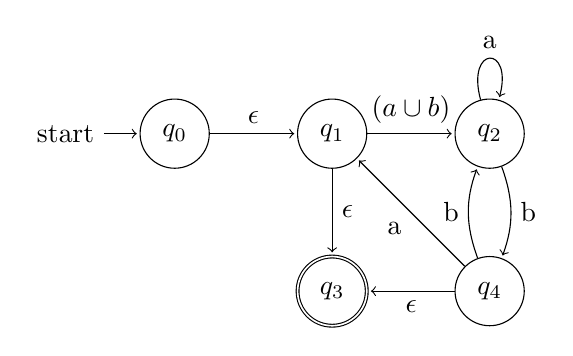
\begin{tikzpicture}[shorten >=1pt,node distance=2cm,on grid,auto] 
        \node[state,initial] (q_0)   {$q_0$}; 
        \node[state] (q_1) [right=of q_0]  {$q_1$};
        \node[state] (q_2) [right=of q_1] {$q_2$}; 
        \node[state,accepting] (q_3) [below=of q_1]  {$q_3$}; 
        \node[state] (q_4)  [right=of q_3] {$q_4$}; 
             \path[->] 
        (q_0) edge node {$\epsilon$} (q_1)
        (q_1) edge node {$(a\cup b)$} (q_2)
        (q_1) edge node {$\epsilon$} (q_3)
        (q_2) edge [loop above] node {a} ()
        (q_2) edge [bend left=20] node {b} (q_4)
        (q_4) edge [bend left=20] node {b} (q_2)
        (q_4) edge node {a} (q_1)
        (q_4) edge node {$\epsilon$} (q_3);
            
    \end{tikzpicture}
\end{center}

\begin{center}

$\Downarrow$

\end{center}

\begin{center}
    \begin{tikzpicture}[shorten >=1pt,node distance=2cm,on grid,auto] 
        \node[state,initial] (q_0)   {$q_0$}; 
        \node[state] (q_2) [right=of q_1] {$q_2$}; 
        \node[state,accepting] (q_3) [below=of q_0]  {$q_3$}; 
        \node[state] (q_4)  [right=of q_3] {$q_4$}; 
             \path[->] 
        (q_0) edge node {$(a\cup b)$} (q_2)
        (q_0) edge node {$\epsilon$} (q_3)
        (q_2) edge [loop above] node {a} ()
        (q_2) edge [bend left=20] node {b} (q_4)
        (q_4) edge [bend left=20] node {$b \cup (a(a \cup b ))$} (q_2)
        (q_4) edge node {$\epsilon \cup a$} (q_3);
            
    \end{tikzpicture}
\end{center}


\end{document}  

